\chapter{Sviluppo Hardware}

\section{Selezione della componentistica}

La realizzazione del progetto richiede un dispositivo embedded con capacità di calcolo sufficiente per eseguire un 
sistema operativo real-time (RTOS) con bassi consumi energetici, connettività' a internet e costi contenuti.

Pertanto la scelta del microcontrollore è ricaduta sulla famiglia di microcontrollori ESP32 prodotta da Espressif Systems~\cite{espressif_website}.
In particolare, il modello scelto, l' ESP32-C3, è un microcontrollore a basso consumo energetico con un'architettura
a core singolo RISC-V~\cite{riscv} a 32 bit, con frequenza di clock fino a 160 MHz, 400 KB di RAM e 384 KB di ROM incorporata.
Esso supporta la connettività Wi-Fi 4 (802.11n) e Bluetooth LE 5.0, dispone, inoltre, di un'unità di crittografia hardware e permette
l'installazione di un sistema operativo real-time come FreeRTOS.

L'architettura RISC-V è risultata essere una scelta ottimale per lo sviluppo di questo framework in quanto
essa è open-source e possiede un'ampia comunità di sviluppatori e una vasta gamma di toolchain e librerie disponibili.

In aggiunta al microcontrollore è stato necessario selezionare un modulo di memoria flash per l'archiviazione dei dati. In 
particolare, è stato scelto il package ESP32-C3-WROOM-02 che include 4 MB di memoria flash, antenne integrate per Wi-Fi e Bluetooth.

\section{Progettazione della development board}

Per utilizzare il microcontrollore ESP32-C3 è stato fondamentale progettare una development board in grado di integrare il package scelto
con i componenti necessari per il funzionamento del dispositivo. In particolare ci si è avvalsi di un connettore USB per la programmazione e l'alimentazione,
di un circuito di alimentazione capace di fornire la corretta tensione per il funzionamento del dispositivo tramite USB o tramite una batteria
ai polimeri di litio (LiPo) e di un corrispettivo circuito di protezione e ricarica della batteria utilizzata.

La development board è stata progettata con il software open-source KiCad~\cite{kicad_website}, adatto alla creazione circuiti stampati in modo semplice e intuitivo.
La scheda è stata disegnata con un layout a due strati con dimensioni di 19x20mm in modo da poter essere facilmente integrata in dispositivi di dimensioni ridotte.

\subsection{Schema elettrico}

Lo schema elettrico della development board consta di tre parti principali esaminate di seguito in dettaglio: l'alimentazione, il microcontrollore e la connettività.

\subsubsection{Alimentazione}

L' alimentazione della development board è stata ideata per essere flessibile e quindi permettere l'utilizzo di una batteria LiPo o di un alimentatore USB.
Data la pericolosità delle batterie LiPo, sì è reso necessario progettare un circuito di protezione in modo da proteggerla e ricaricala in modo sicuro.
Inoltre, le tensioni fornite dalla batteria LiPo(comprese in un range che va da 3.2V a 4.2V) e dall'alimentatore USB (5V) 
sono state regolate a 3.3V per il corretto funzionamento del microcontrollore.

\begin{figure}[H]
  \centering
  \includegraphics[width=0.8\textwidth]{images/chapter2/charging.png}
  \caption{Circuito di ricarica della batteria}
  \label{fig:charging}
\end{figure}

L'immagine mostra le connessioni necessarie per il funzionamento del IC TP4057~\cite{charger_sheet} in grado di ricaricare la batteria con una corrente 
massima di 500mA utilizzando la tensione di 5V fornita dal connettore USB-C.

\begin{figure}[H]
  \centering
  \includegraphics[width=0.8\textwidth]{images/chapter2/protection.png}
  \caption{Circuito di protezione della batteria}
  \label{fig:protection}
\end{figure}

Per proteggere la batteria da sovraccarichi e sovrascariche è stato utilizzato il circuito integrato FM2113~\cite{protection_sheet} che
monitora la tensione della batteria e ne interrompe la carica o la scarica in caso di tensioni non sicure.

\begin{figure}[H]
  \centering
  \includegraphics[width=0.8\textwidth]{images/chapter2/regulator.png}
  \caption{Circuito di regolazione del voltaggio}
  \label{fig:regulator}
\end{figure}

Per alimentare il microcontrollore è stato scelto il regolatore di tensione della Texas Instruments 1~\cite{regulator_sheet} 
che è in grado di convertire con un alto grado di efficienza energetica la tensione della batteria a 3.3V, necessaria per il funzionamento del microcontrollore.

\subsubsection{Microcontrollore}

\begin{figure}[H]
  \centering
  \begin{minipage}[b]{0.70\textwidth}
    \includegraphics[width=1.0\textwidth]{images/chapter2/mcu.png}
    \caption{Collegamento del microcontrollore}
    \label{fig:mcu}  
  \end{minipage}
  \hfill
  \begin{minipage}[b]{0.28\textwidth}
    \includegraphics[width=1.0\textwidth]{images/chapter2/divider.png}
    \caption{Partitore di tensione}
    \label{fig:divider}
    \end{minipage}
\end{figure}

Il package ESP32-C3-WROOM-02~\cite{esp32_c3_wroom_02_sheet} è stato collegato al circuito di alimentazione e ai componenti necessari per il suo funzionamento,
ovvero i condensatori di disaccoppiamento e un partitore di tensione per il monitoraggio della tensione della batteria.

\subsubsection{Connettività}

\begin{figure}[H]
  \centering
  \includegraphics[width=0.8\textwidth]{images/chapter2/usb.png}
  \caption{Connettore USB-C}
  \label{fig:usb}
\end{figure}
Il connettore USB-C è stato scelto per la sua versatilità e la sua diffusione. Viene utilizzato per alimentare il 
dispositivo e programmarlo.

Per poter collegare sensori e attuatori esterni al microcontrollore sono stati aggiunti due connettori 
per le porte General Purpose Input/Output (GPIO) del microprocessore.

\subsection{Layout PCB}

\begin{figure}[H]
  \centering
  \includegraphics[width=0.5\textwidth]{images/chapter2/pcb.png}
  \caption{Layout del PCB}
  \label{fig:pcb}
\end{figure}

Il layout del PCB è stato disegnato in modo da minimizzare i costi di produzione e di assemblaggio:
esso sfrutta un layout a due strati con componenti montati solo sul lato superiore.

Il layer inferiore viene utilizzato per le piste di alimentazione e di massa, mentre il layer superiore 
per i segnali e i componenti.

Grazie al check delle regole di progettazione di KiCad è stato possibile verificare la correttezza del 
layout e la presenza di eventuali errori prima ancora di inviare il PCB in produzione.
\subsection{Manufacturing}

Il PCB è stato fabbricato tramite il servizio online JLCPCB~\cite{jlcpcb}, atto alla produzione economica e veloce di circuiti stampati.
Questo stesso servizio consente l'assemblaggio dei componenti sulla scheda, step necessario per ottenere un prodotto finito.

\begin{figure}[H]
  \centering
  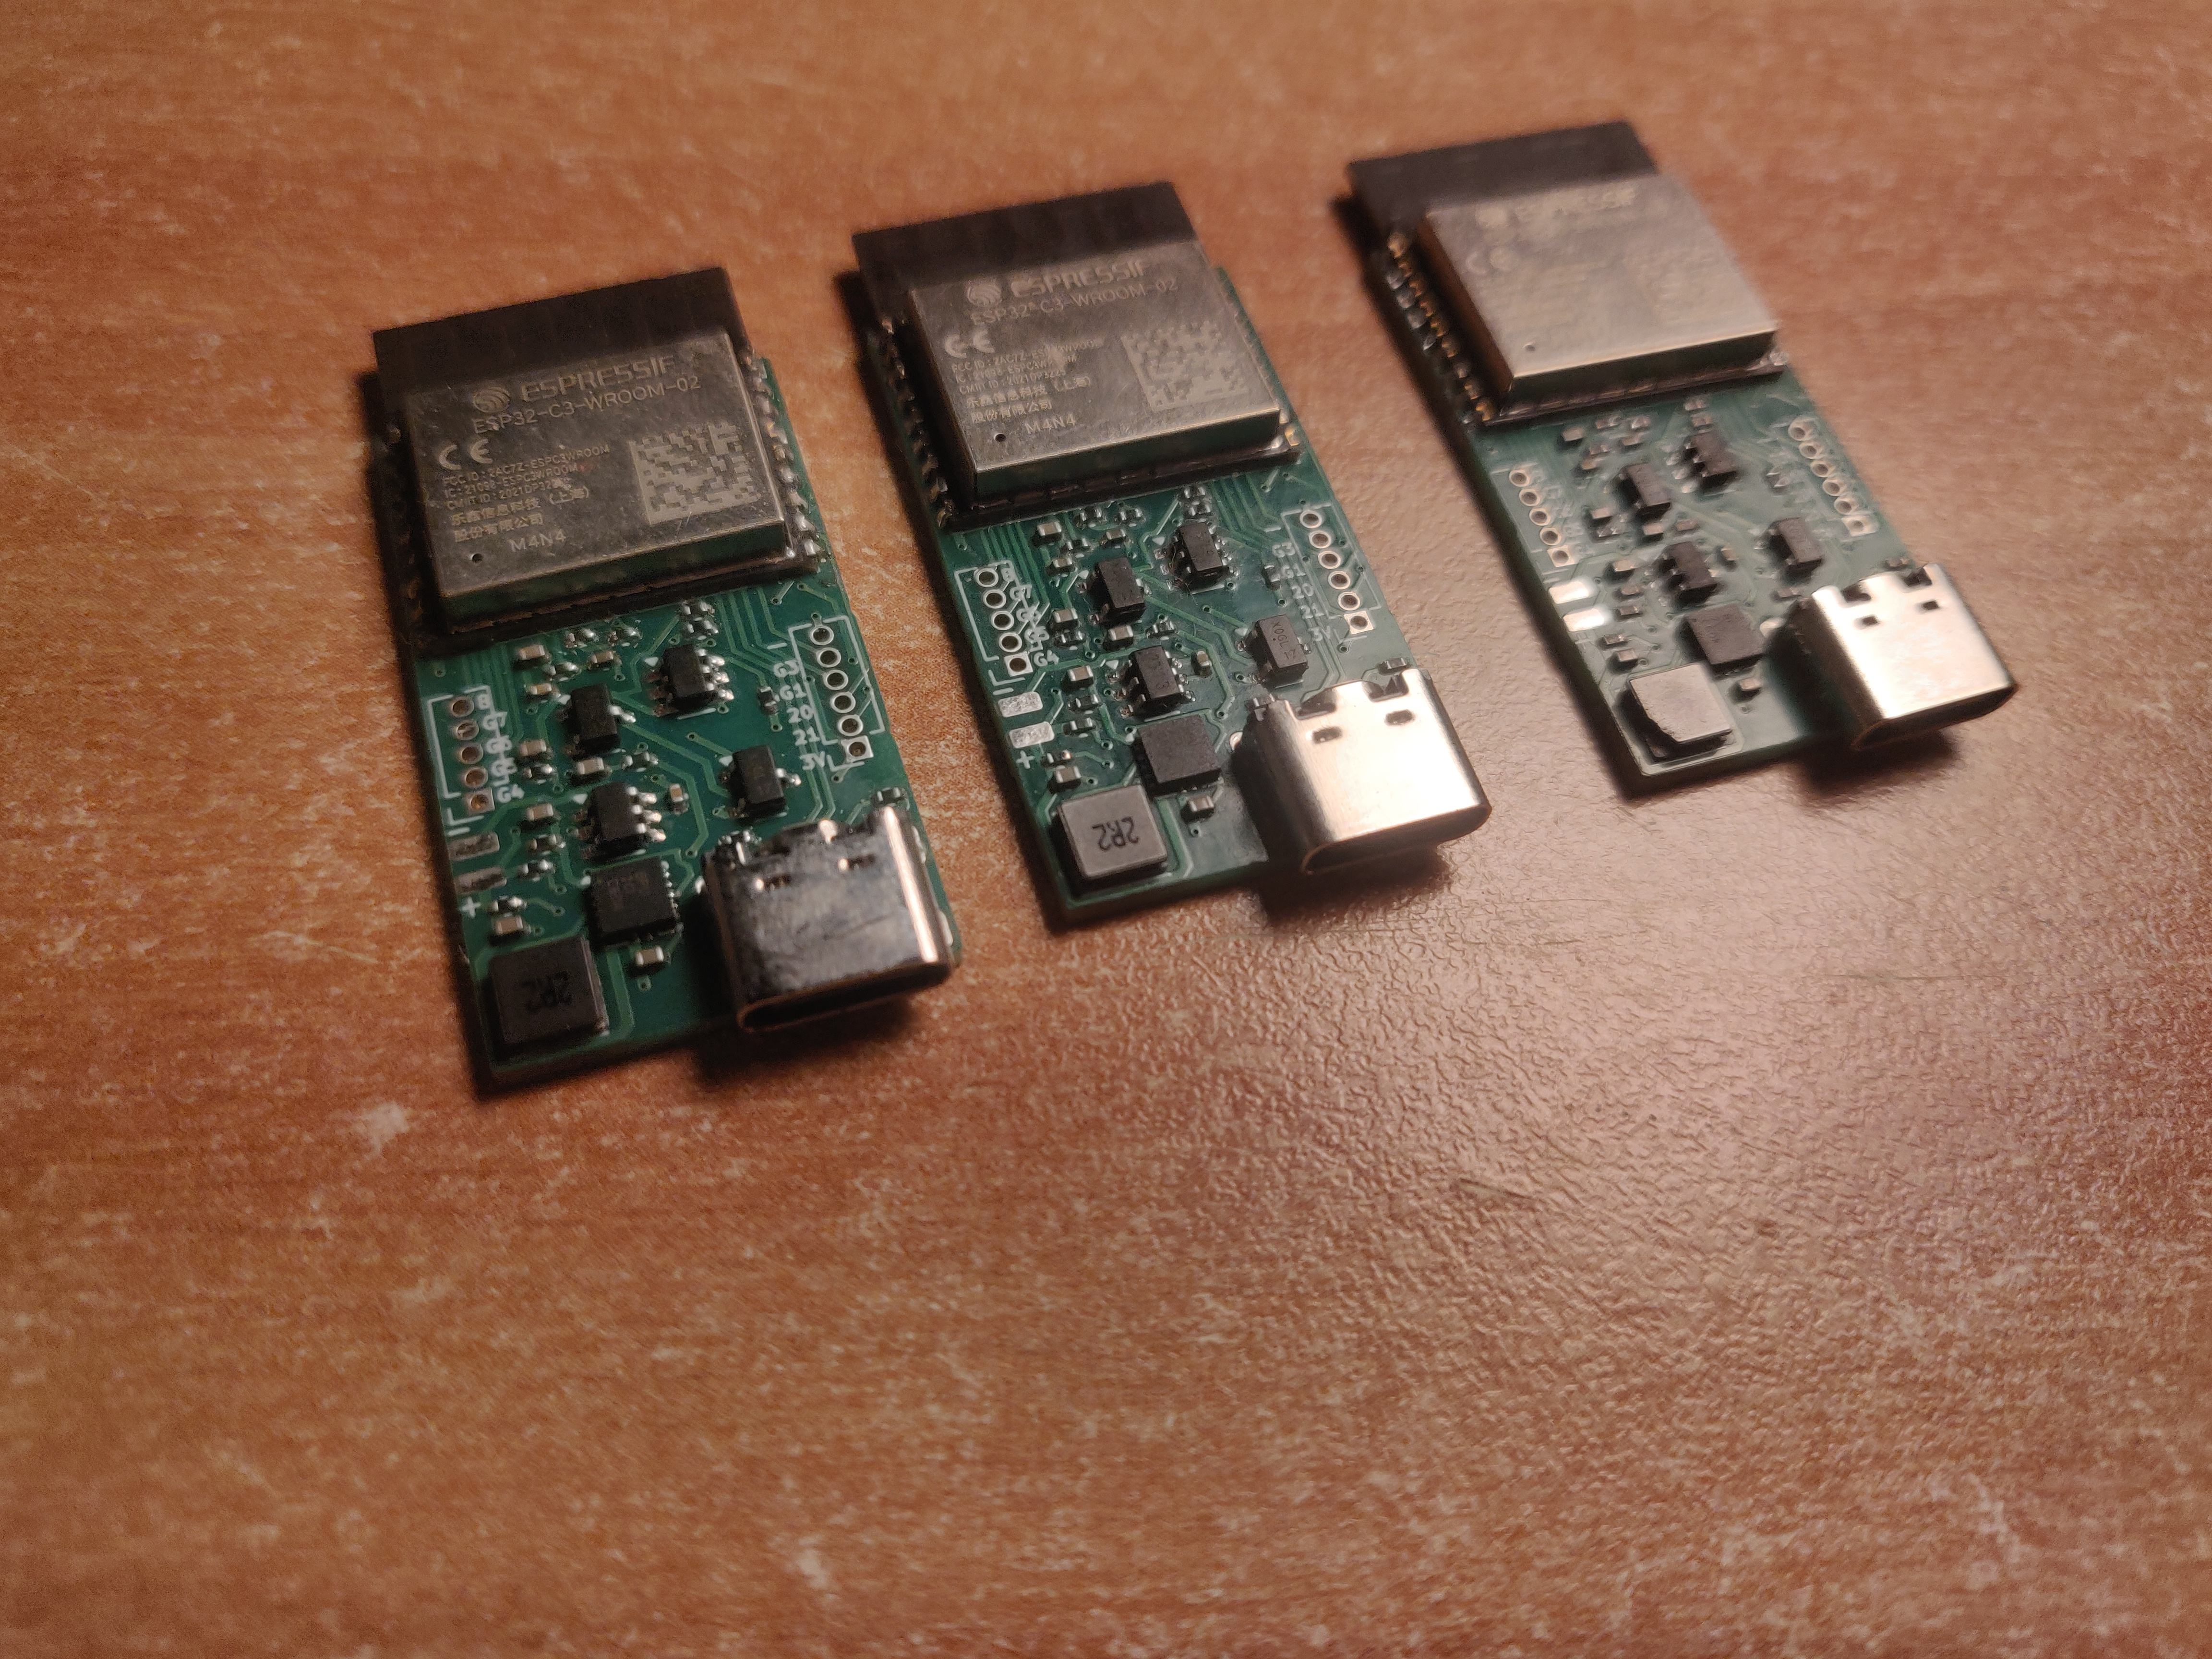
\includegraphics[width=0.6\textwidth]{images/chapter2/board.jpg}
  \caption{PCB assemblato}
  \label{fig:board}
\end{figure}

\section{Progettazione prototipo embedded}

Il corretto funzionamento della development board è stato testato attraverso la progettazione di un prototipo di 
dispositivo embedded funzionante.
Per raggiungere tale obiettivo ci si è avvalsi di un dispositivo già esistente, 
ovvero delle lampade da notte RGB in silicone dotate di sensore di shock, modificandole e adattandole alle nostre esigenze.

\subsection{Reverse engineering del device}

\begin{figure}[H]
  \centering
  \includegraphics[width=0.6\textwidth]{images/chapter2/step0.jpg}
  \caption{Scheda originale}
  \label{fig:original_pcb}
\end{figure}

Il dispositivo originale era composto da una scheda con un microcontrollore generico, 4 MOSFET per il controllo dei led 
(una coppia di led RGB e una coppia di led bianchi) e un sensore di shock.

Si è proceduto con il reverse engineering della scheda per poter comprendere il funzionamento del dispositivo e successivamente modificarlo.
L'utilizzo di un tester è stato essenziale per identificare i pin di controllo dei led ed il funzionamento del sensore.

\begin{figure}[H]
  \centering
  \begin{minipage}[b]{0.45\textwidth}
    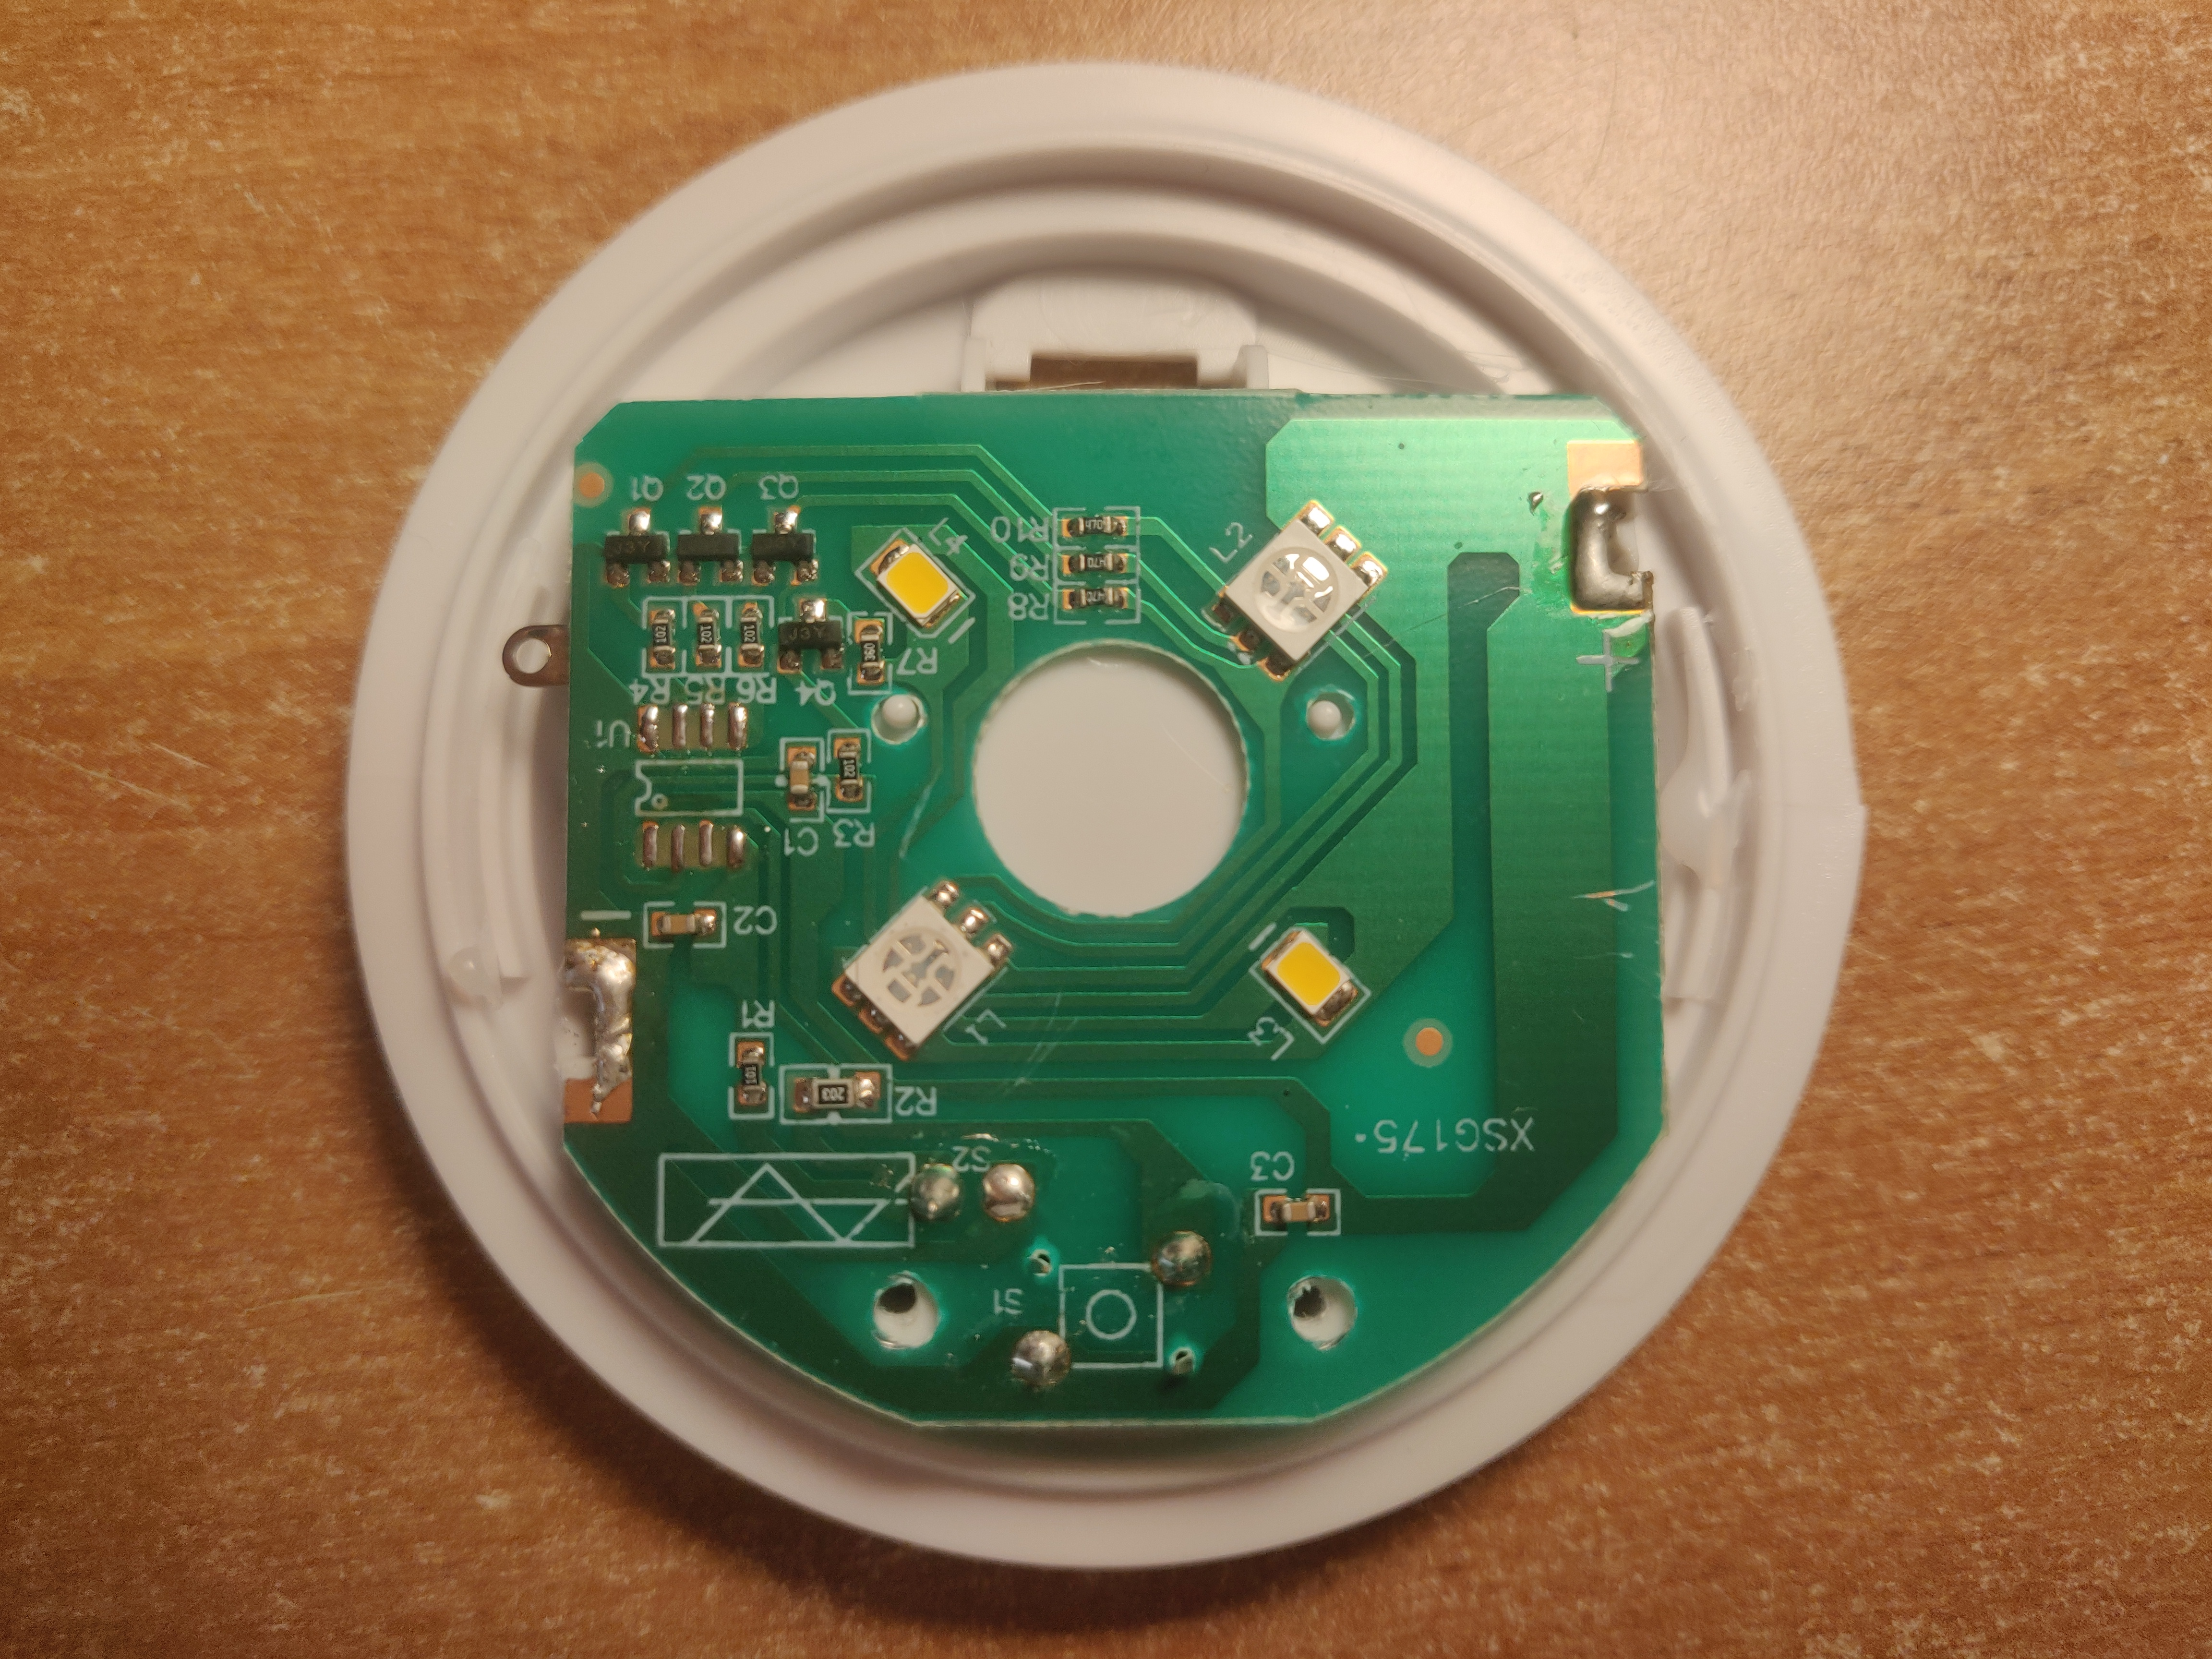
\includegraphics[width=1.0\textwidth]{images/chapter2/step1.jpg}
    \caption{Step 1: rimozione del processore}
    \label{fig:step1}
  \end{minipage}
  \hfill
  \begin{minipage}[b]{0.45\textwidth}
    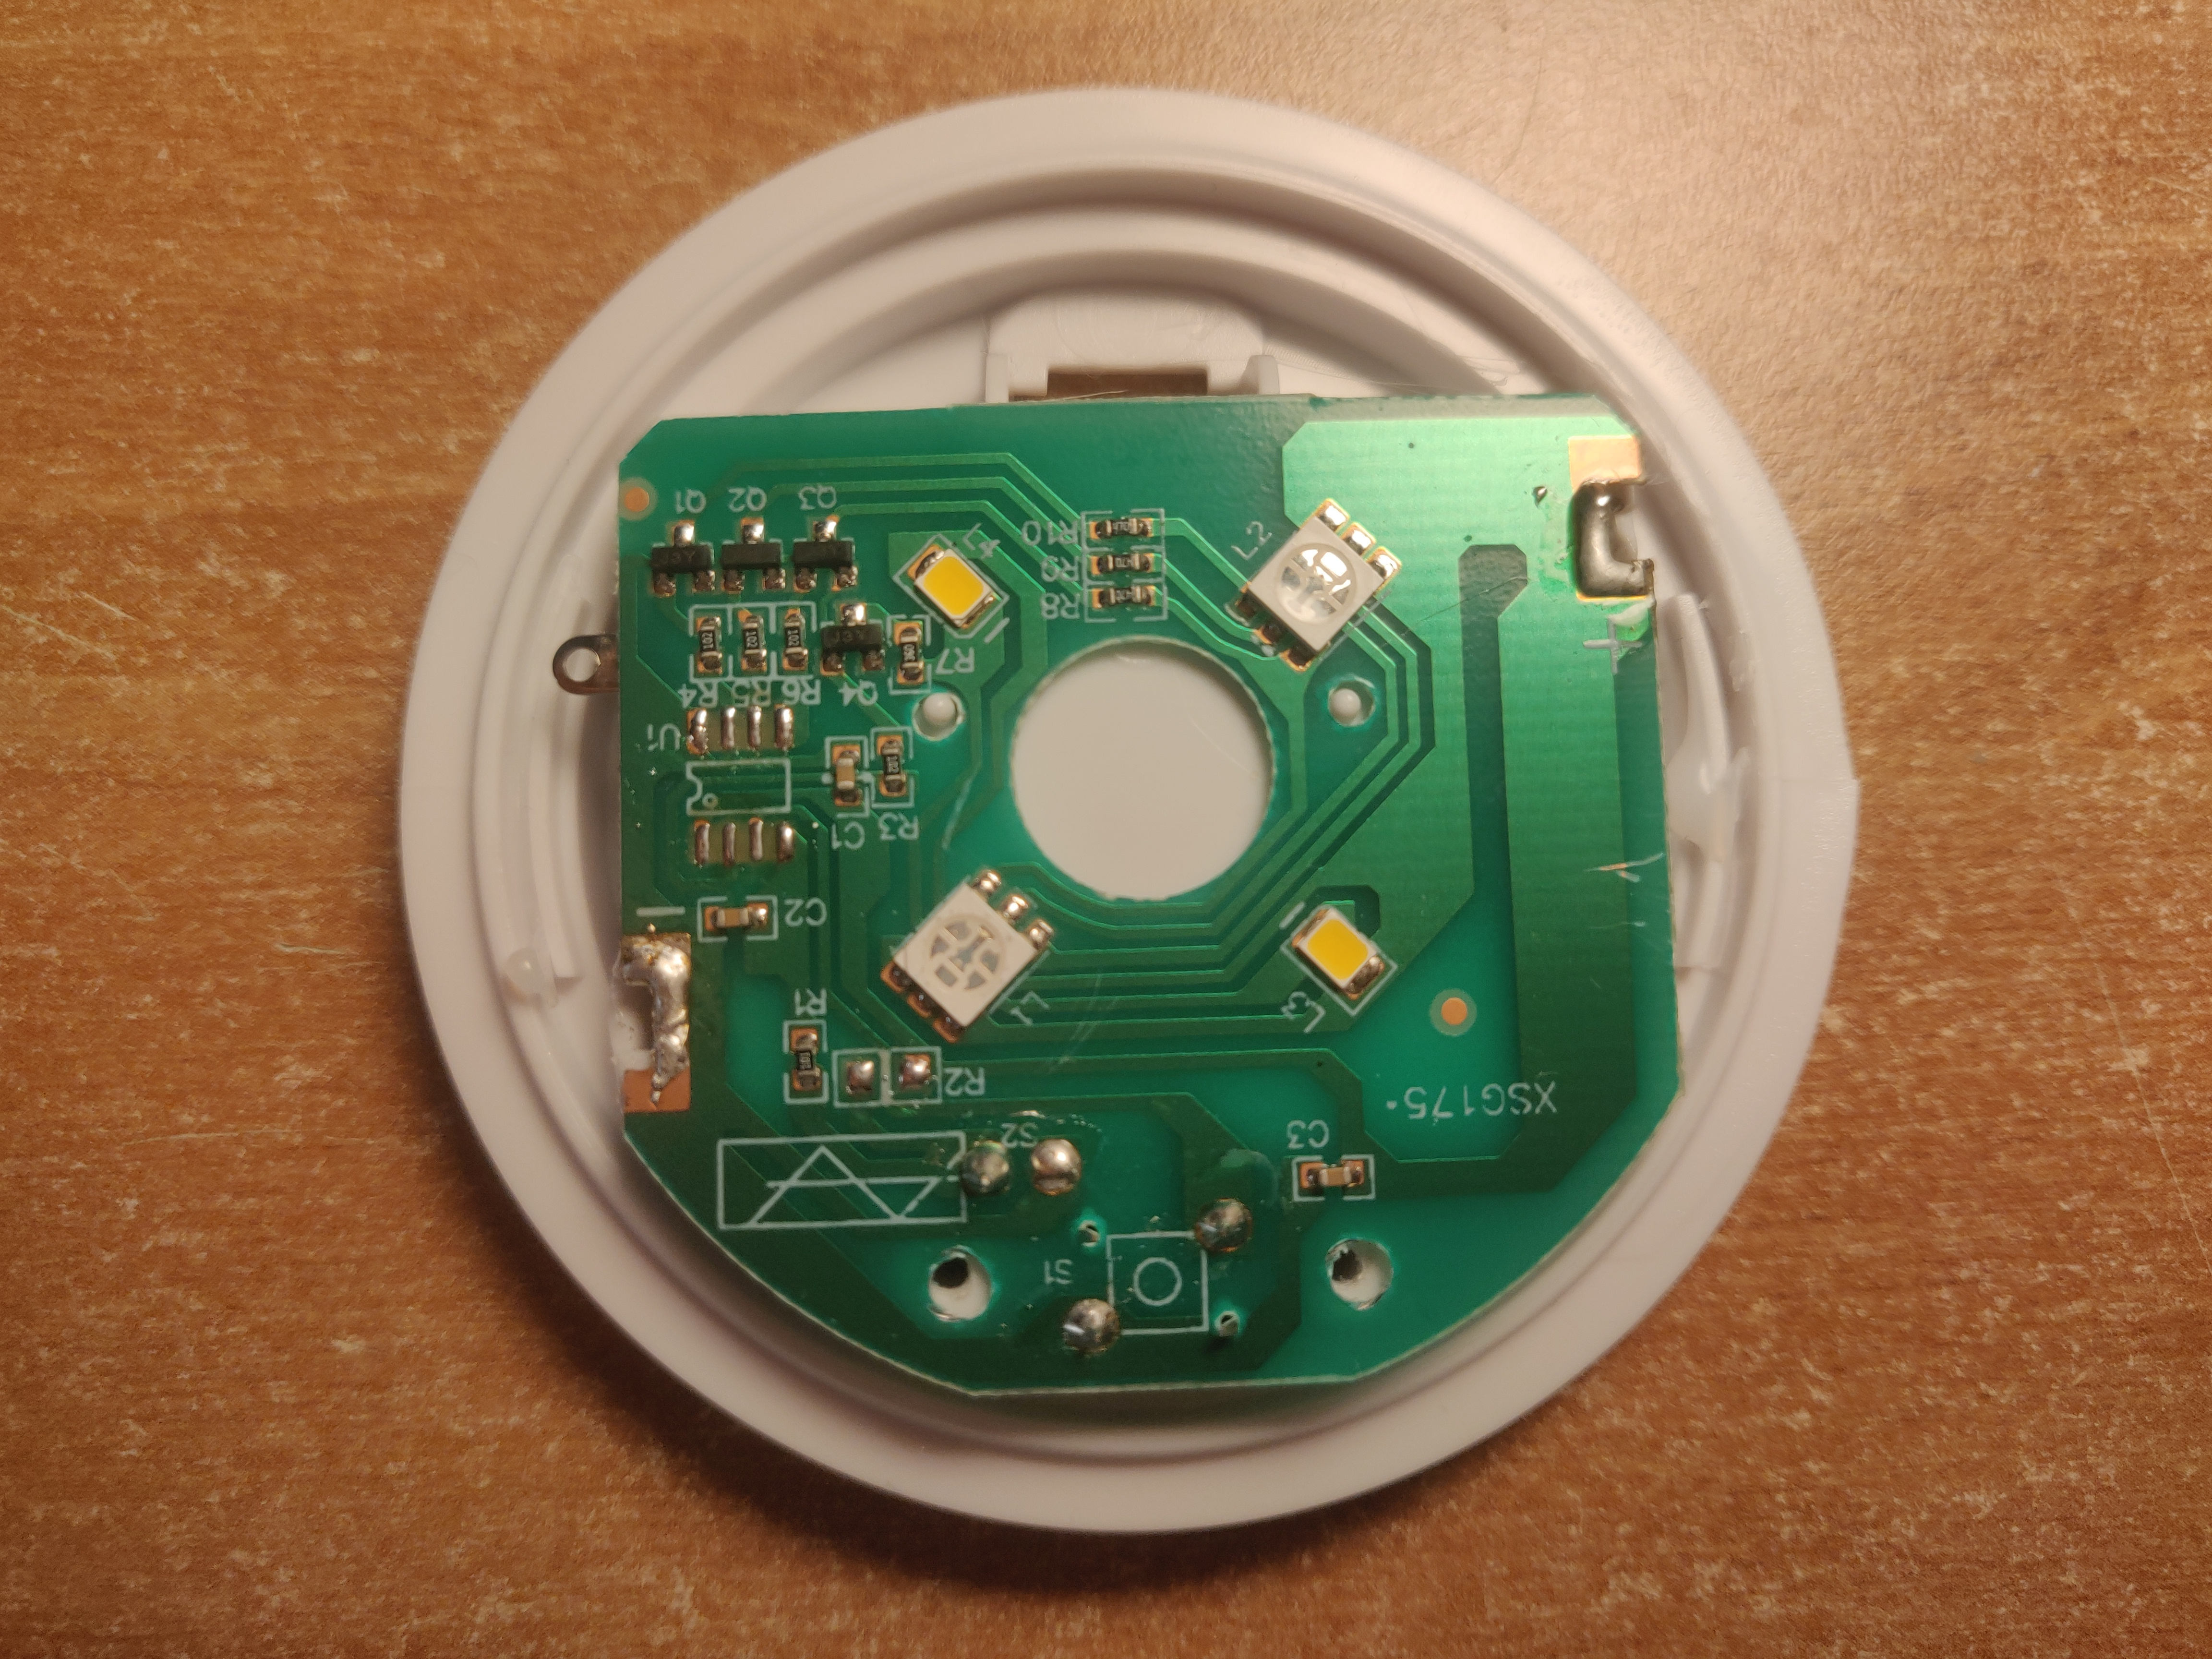
\includegraphics[width=1.0\textwidth]{images/chapter2/step2.jpg}
    \caption{Step 2: rimozione del resistore R2}
    \label{fig:step2}
    \end{minipage}
\end{figure}

\begin{figure}[H]
  \centering
  \begin{minipage}[b]{0.45\textwidth}
    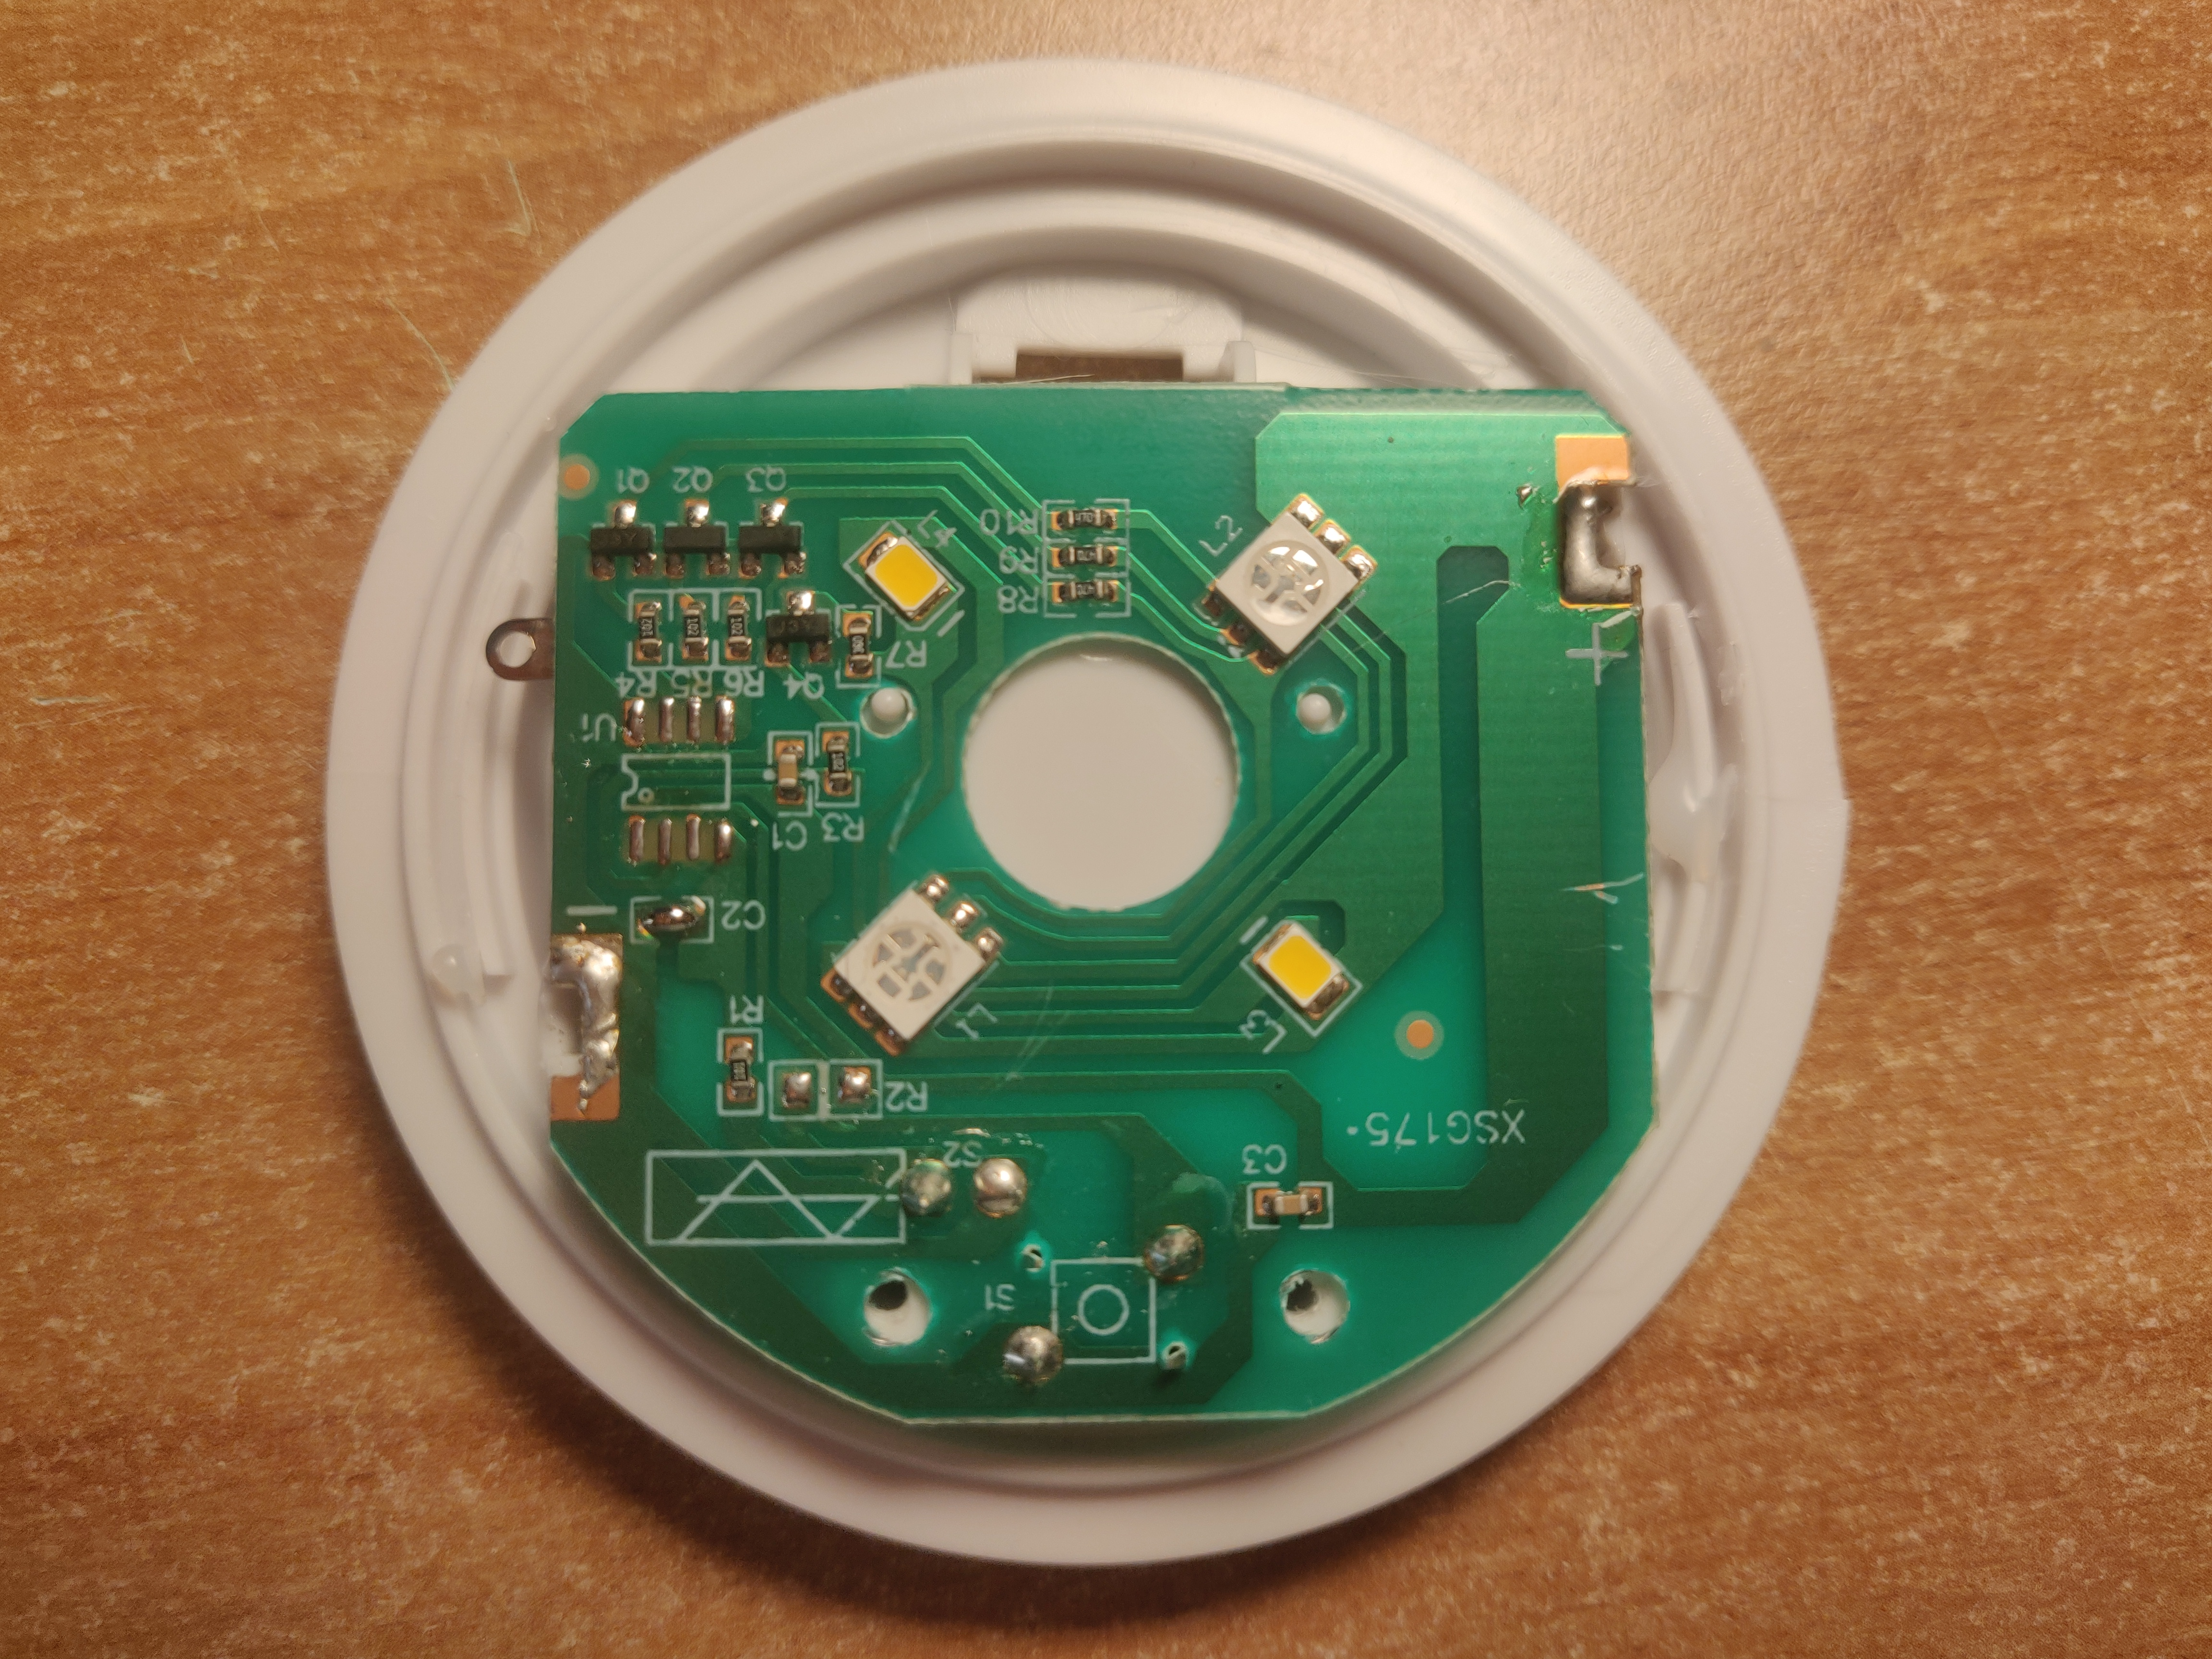
\includegraphics[width=1.0\textwidth]{images/chapter2/step3.jpg}
    \caption{Step 3: rimozione del condensatore C2 e cortocircuitazione dei pad}
    \label{fig:step2}  
  \end{minipage}
  \hfill
  \begin{minipage}[b]{0.45\textwidth}
    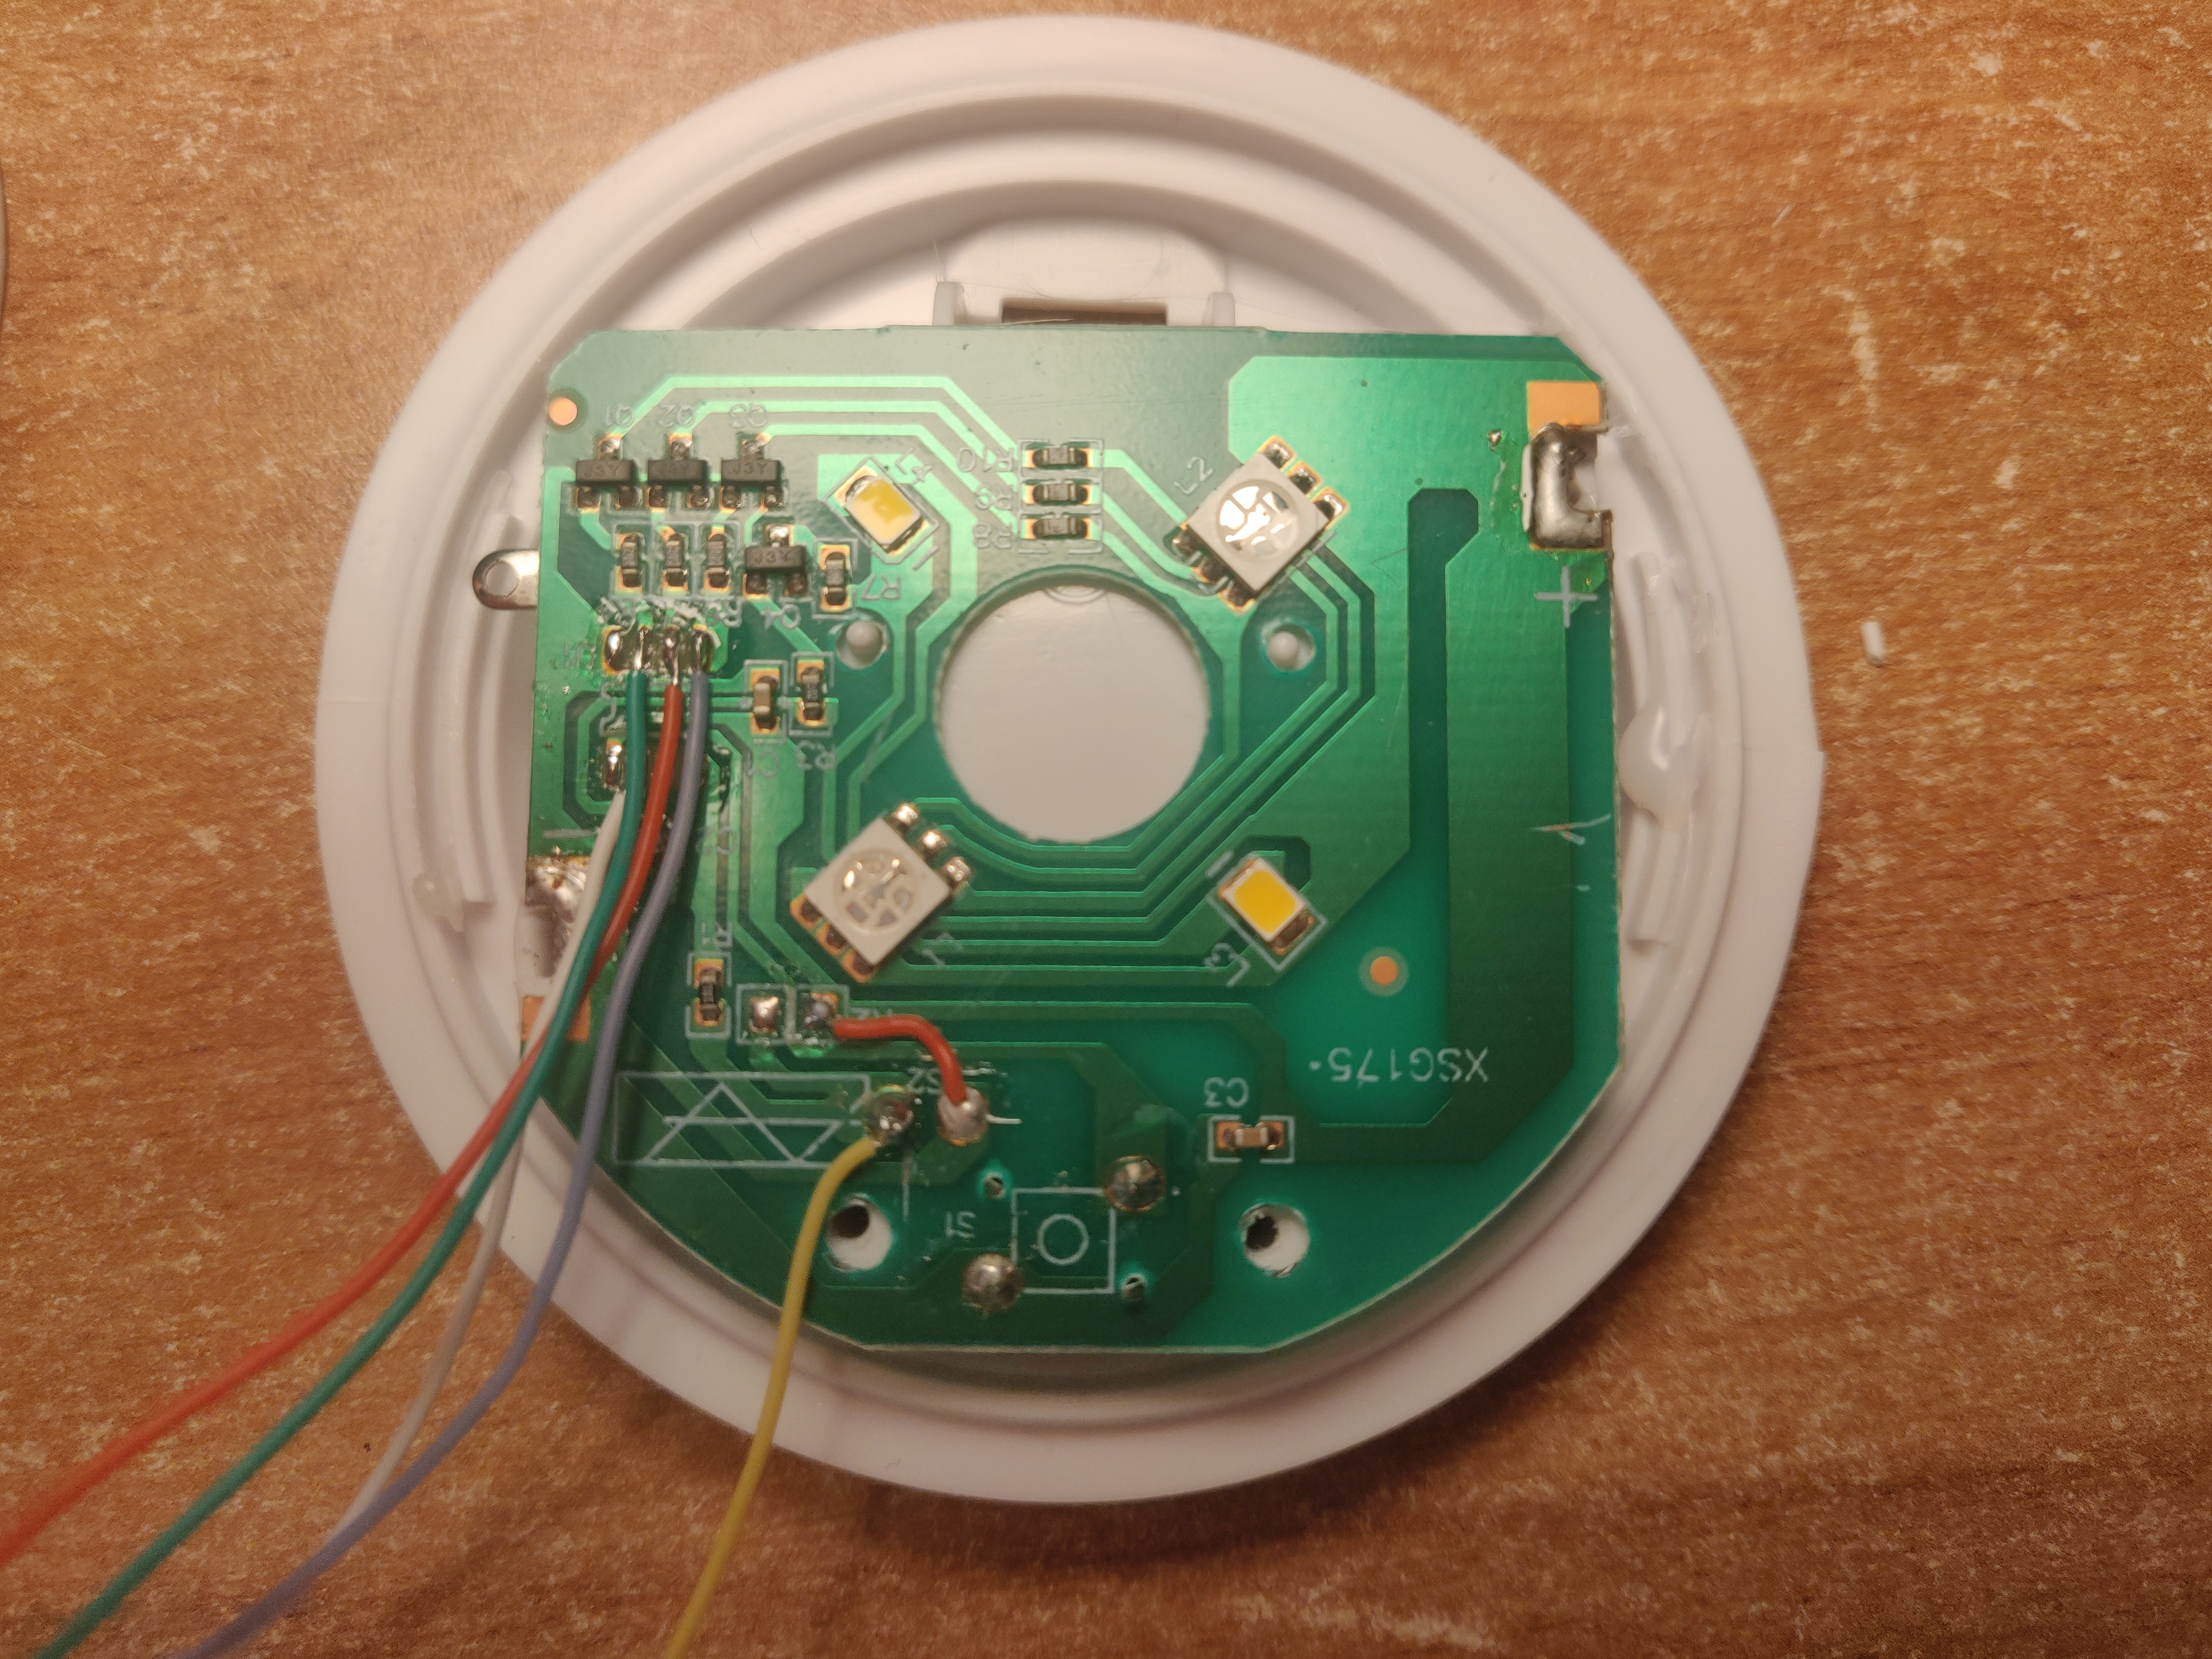
\includegraphics[width=1.0\textwidth]{images/chapter2/step4.jpg}
    \caption{Step 4: saldatura cavi per controllare le periferiche}
    \label{fig:step2}
      \end{minipage}
\end{figure}

\subsection{Creazione del prototipo}

Dopo aver disegnato lo schema elettrico della scheda originale e dissaldato il microcontrollore presente, si è proceduto
con la sostituzione di quest'ultimo con la development board precedentemente progettata.

Successivamente, è stato necessario creare un alloggiamento per la development board e la nuova batteria LiPo e stamparlo in 3D.
Il disegno dell'enclosure è stato elaborato usando il software Fusion 360~\cite{fusion360} mentre lo slicing è avvenuto tramite Ultimaker Cura~\cite{cura}.

\begin{figure}[H]
  \centering
  \begin{minipage}[b]{0.68\textwidth}
    \includegraphics[width=1.0\textwidth]{images/chapter2/fusion360.png}
    \caption{Rendering dell'alloggiamento su Fusion360}
    \label{fig:fusion360}
    \end{minipage}
  \hfill
  \begin{minipage}[b]{0.3\textwidth}
    \includegraphics[width=1.0\textwidth]{images/chapter2/step5.jpg}
    \caption{Installazione della board e della batteria nell'alloggiamento}
    \label{fig:step5}  
      \end{minipage}
\end{figure}

In tal modo si è ottenuto un dispositivo embedded perfettamente in grado di testare il corretto funzionamento del framework sviluppato nella tesi.